\documentclass[10pt,a4paper]{article}
\usepackage[utf8]{inputenc}
\usepackage[english]{babel}
\usepackage{amsmath}
\usepackage{amsfonts}
\usepackage{amssymb}
\usepackage{graphicx}
\usepackage[left=2cm,right=2cm,top=2cm,bottom=2cm]{geometry}

\usepackage{setspace}
\setstretch{1.5}

\usepackage{float}
    
\renewcommand{\familydefault}{phv}

\usepackage[colorlinks=true,
			urlcolor=cyan,
			linkcolor=black]{hyperref}
			
\graphicspath{{figures/}}

\title{H1N1 and Seasonal Flu Vaccine Prediction\\
\Large Data Science Intro Project}

\begin{document}
\maketitle

\begin{abstract}
   In this project I try to predict a subject's probability of taking the H1N1 and seasonal flue vaccines from the input data provided by the competition.
   I use an iterative approach based on gathering insight from data using EDA, performing the preprocessing of the data, selecting the best model to be used with the data, tuning that same model (or models) and then joining every step to make my final predictions.
   The final model was chosen as a stacking classifier of different models which performed in the top 14\% of participants with an AUROC of 0.8442.
\end{abstract}

\tableofcontents

\pagebreak
\section{Introduction}

The aim of this report is to provide insight into the framework I used to achieve a top 14\% entry to the competition \href{https://www.drivendata.org/competitions/66/flu-shot-learning/}{Flu Shot Learning: Predict H1N1 and Seasonal Flu Vaccines}.

I began by looking at the competition problem description.

\subsection{Competition Objective}

The objective of the competition is to predict the probability of an individual to take their H1N1 and seasonal flu vaccines. This puts the problem as a multilabel classification one where we have to predict two labels: \textit{h1n1\_vaccine} and \textit{seasonal\_vaccine}.

It is important to notice that both labels are binary and any combination of the two for each individual is possible.

\subsection{Dataset Features}

The dataset is composed of 36 columns in which one of them is the \textit{respondent\_id} which identifies the individual and the remaining 35 are features we can use in modeling.

Among these features we have multiple regarding the individual's opinion, behaviour, etc. regarding the deseases as well as some socio-economic features. I will not get into detail on each feature here since I will explain some of them further in Sec. \ref{sec:eda}.

For now, it is sufficient we know that there are both numerical and categorical variables - which will need to be encoded before modeling.

\subsection{Evaluation Metric}

The metric used to evaluate the result of the model predictions is the area under the receiver operating characteristic curve (AUROC).

\begin{figure}[H]
\centering
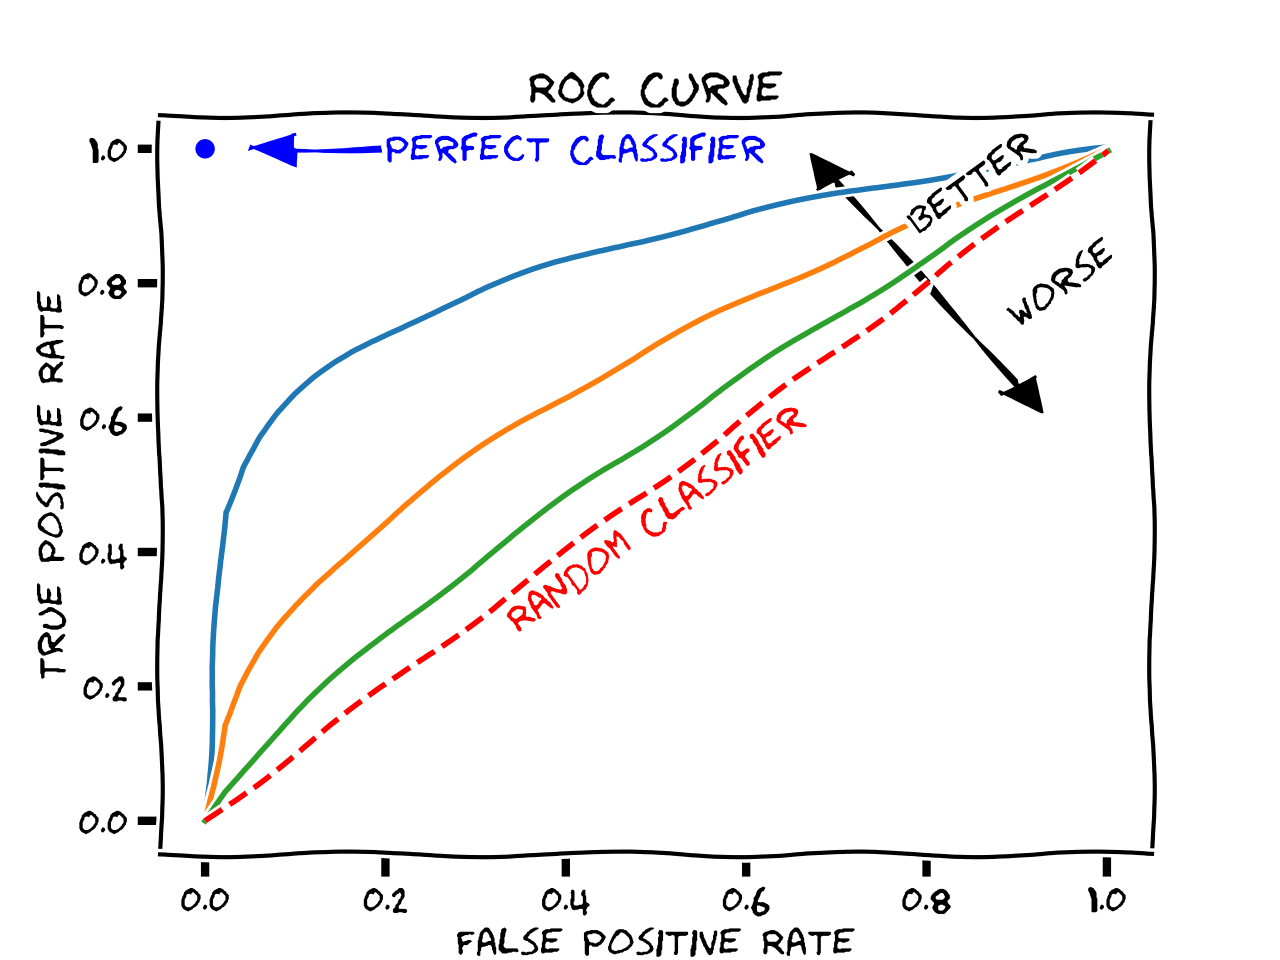
\includegraphics[scale=0.2]{auroc.png}
\label{fig:auroc}
\caption{AUROC evaluation metric. \href{https://commons.wikimedia.org/wiki/File:Roc-draft-xkcd-style.svg}{[1]}}
\end{figure}

This metric calculates the area under curves such as the ones in Fig. \ref{fig:auroc}. The curves are a plot of the model true positive rate (TPR) vs its false positive rate (FPR). Thus, the curve for a random classifier is a straight line at a slope of 1 and the perfect classifier is a single point with $TPR = 1$ and $FPR = 0$. As such, the AUROC for a random classifier is $0.5$ and the AUROC of a perfect classifier is $1$. Taking this into account we see that we want to increase our model's AUROC, to increase its accuracy.

\section{Solution Approach}

\section{Exploratory Data Analysis}\label{sec:eda}

\section{Model Selection}

\section{Model Tuning}

\section{Model Fitting and Predictions}

\section{Conclusions and Future Work}

\end{document}